\documentclass[aspectratio=169,11pt]{beamer}

\usetheme{Madrid}
\usecolortheme{seahorse}

\usepackage{amsmath,amssymb}
\usepackage{booktabs}
\usepackage{array}
\usepackage{graphicx}

\title{BIOS 662 Review}
\author{Chenghao Wang}
\institute{BIOS 662: Intermediate Statistical Methods}
\date{September 28, 2026}

\setbeamertemplate{navigation symbols}{}
\setbeamertemplate{footline}[frame number]

\newcommand{\E}{\operatorname{E}}
\newcommand{\Var}{\operatorname{Var}}

\begin{document}

\begin{frame}
  \titlepage
\end{frame}

\begin{frame}{Today's questions}
  \begin{enumerate}
    \item How do parallel group and crossover designs differ?
    \item What is the purpose of each clinical-trial phase?
    \item What does ``sample size'' mean in a bootstrap?
    \item When should we use an exact method rather than a large-sample method?
    \item How do we construct a confidence interval for a population median?
  \end{enumerate}
  \vfill
  \alert{Goal:} connect the definitions to the choice of a statistical method.
\end{frame}

\section{Study designs}

\begin{frame}{Parallel group design}
  \begin{columns}[T]
    \column{0.55\textwidth}

      Each participant is randomized to one treatment and remains on it.

      \[
        \text{Group 1: } A \qquad \text{Group 2: } B
      \]
      A common estimand is the between-group mean difference
      \[
        \Delta = \E(Y\mid A)-\E(Y\mid B).
      \]
    \column{0.42\textwidth}
      \begin{exampleblock}{Pros}
        \begin{itemize}
          \item Simple analysis and interpretation
          \item No carryover between treatments
          \item Takes shorter time than crossover design
          \item Suitable for permanent or lasting effects
        \end{itemize}
      \end{exampleblock}
      \begin{alertblock}{Cons}
        Between-person variability contributes to the variance.
      \end{alertblock}
  \end{columns}
\end{frame}

\begin{frame}{Crossover design}
  \begin{columns}[T]
    \column{0.54\textwidth}
      Participants receive multiple treatments in randomized sequences:
      \[
        \text{Sequence 1: } A \longrightarrow B,
        \qquad
        \text{Sequence 2: } B \longrightarrow A.
      \]
      With two periods, a natural contrast is within participant:
      \[
        \Delta = \E(Y_A-Y_B).
      \]
      Each participant serves as their own control, eliminating
      subject-to-subject variability.

      Why randomizing the sequence? To adjust for period effects.
    \column{0.43\textwidth}
      \footnotesize
      \begin{exampleblock}{Pros}
        Removes much between-subject variation, often increasing efficiency.
      \end{exampleblock}
      \vspace{-0.4em}
      \begin{alertblock}{Cons}
        \begin{itemize}
          \setlength{\itemsep}{0pt}
          \item Carryover effects: the effect of an earlier treatment persists
                into a later period.
          \item Calendar-time effects: outcome changes due to real-world time rather than
                the treatment.
          \item The treatment introduces permanent changes to the experimental units.
          \item Takes longer time than parallel group design:
                the chance of dropout increases; the investigator and subject
                enthusiasm wanes.
        \end{itemize}
      \end{alertblock}
  \end{columns}
\end{frame}

\begin{frame}{Parallel or crossover?}
  \small
  \begin{tabular}{>{\raggedright\arraybackslash}p{0.24\textwidth}
                  >{\raggedright\arraybackslash}p{0.33\textwidth}
                  >{\raggedright\arraybackslash}p{0.33\textwidth}}
    \toprule
    & \textbf{Parallel} & \textbf{Crossover} \\
    \midrule
    Best fit & Lasting treatment effects; unstable disease & Reversible effects; stable condition \\
    Comparison & Between participants & Within participants \\
    Main concern & Baseline heterogeneity & Carryover and period effects \\
    Washout & Not needed & Needed when residual effects are plausible \\
    \bottomrule
  \end{tabular}

  \vspace{0.7em}
  \begin{exampleblock}{Example}
    For something like blood-pressure drugs with short-lived effects, crossover can be useful.
    For surgery, vaccines, cancer treatment, or therapies that permanently change disease course,
    parallel design is usually a better choice.
  \end{exampleblock}

  \textbf{Check:} Why can increasing the washout period reduce carryover but increase dropout?
\end{frame}

\section{Clinical-trial phases}

\begin{frame}{Clinical-trial phases I and II}
  \begin{columns}[T]
    \column{0.49\textwidth}
      \begin{block}{Phase I: safety and dose}
        \begin{itemize}
          \item Primary focus: safe dosage range, side effects, and pharmacokinetics
          \item If possible, gain early evidence of effectiveness
          \item Usually a small group of people (20-80)
          \item Often healthy volunteers; sometimes patients
        \end{itemize}
      \end{block}
    \column{0.49\textwidth}
      \begin{block}{Phase II: preliminary efficacy}
        \begin{itemize}
          \item Effectiveness plus continued safety assessment
          \item A larger group of people (100-300)
          \item Patients with the condition of interest
        \end{itemize}
      \end{block}
  \end{columns}
  \vfill
  \alert{The phase describes the development objective, not merely the sample size.}

  Cell/lab studies and animal studies are performed before the clinical trial (pre-clinical research).

\end{frame}

\begin{frame}{Clinical-trial phases III and IV}
  \begin{columns}[T]
    \column{0.49\textwidth}
      \begin{block}{Phase III: confirmatory evaluation}
        \begin{itemize}
          \item Further evaluation of effectiveness and safety
          \item Larger populations (1000-3000) and in different regions and countries
        \end{itemize}
      \end{block}
    \column{0.49\textwidth}
      \begin{block}{Phase IV: after approval}
        \begin{itemize}
          \item After approval
          \item Long-term outcomes and uncommon adverse events
          \item In the general population over a longer timeframe
        \end{itemize}
      \end{block}
  \end{columns}
  \vspace{0.6em}
  \begin{alertblock}{Classification is not always clean}
    The phase framework is most natural for drug development. Trials of behavioral,
    surgical, or already-approved interventions may not fit one phase exactly.
  \end{alertblock}
  \textbf{Check:} A large definitive trial of an already-approved device resembles
  Phase III in purpose, but why might the label be debatable?
\end{frame}

\section{Bootstrap sample size}

\begin{frame}{Three quantities that may be easy to confuse}
  \begin{center}
  \begin{tabular}{>{\raggedright\arraybackslash}p{0.19\textwidth}
                  >{\raggedright\arraybackslash}p{0.34\textwidth}
                  >{\raggedright\arraybackslash}p{0.36\textwidth}}
    \toprule
    \textbf{Quantity} & \textbf{Meaning} & \textbf{What it controls} \\
    \midrule
    Original \(n\) & Number of independent observations collected & Statistical information about the population \\
    Resample size \(n^*\) & Observations drawn with replacement in one bootstrap sample & Usually set to \(n\) to mimic sampling from the empirical distribution \\
    Replicates \(B\) & Number of bootstrap samples generated & Monte Carlo stability of the bootstrap calculation \\
    \bottomrule
  \end{tabular}
  \end{center}
  \vfill
  Increasing \(B\) reduces simulation noise at approximately the rate \(B^{-1/2}\),
  but it does \alert{not} add information to the original study.
\end{frame}

\begin{frame}{A bootstrap algorithm}
  Given observations \(x_1,\ldots,x_n\) and statistic
  \(\widehat\theta=t(x_1,\ldots,x_n)\):
  \begin{enumerate}
    \item For \(b=1,\ldots,B\), sample \(n\) observations with replacement from
          \(\{x_1,\ldots,x_n\}\).
    \item Compute the statistic \(\widehat\theta^{*(b)}\) from bootstrap sample \(b\).
    \item Use the empirical distribution
          \(\widehat\theta^{*(1)},\ldots,\widehat\theta^{*(B)}\)
          to estimate uncertainty.
  \end{enumerate}
  \begin{block}{For a bootstrap-\(t\) interval}
    Studentize each replicate:
    \[
      Z^{*(b)}=\frac{\widehat\theta^{*(b)}-\widehat\theta}
                       {\widehat{\operatorname{se}}^{*(b)}}.
    \]
    Quantiles of the \(Z^{*(b)}\)'s replace normal or \(t\) critical values.
  \end{block}
\end{frame}

\begin{frame}{How large should \(B\) be?}
  \begin{itemize}
    \item The course examples use \(B=500\), which is enough to demonstrate the method.
    \item Other common choices of \(B\): 1000, 2000, 5000, 10000.
    \item Compute \(B\) using the error rate \(B^{-1/2}\).
  \end{itemize}
  \begin{alertblock}{What increasing \(B\) cannot fix}
    Bias, small original sample sizen $n$, a poor bootstrap approximation
    (for statistics such as extreme quantiles).
  \end{alertblock}
  \textbf{Check:} If \(n=21\) and \(B=2000\), how many observations are in each
  ordinary nonparametric bootstrap sample?
\end{frame}

\section{Exact and large-sample inference}

\begin{frame}{Exact versus large-sample methods}
  \small
  \begin{tabular}{>{\raggedright\arraybackslash}p{0.21\textwidth}
                  >{\raggedright\arraybackslash}p{0.34\textwidth}
                  >{\raggedright\arraybackslash}p{0.34\textwidth}}
    \toprule
    & \textbf{Exact method} & \textbf{Large-sample method} \\
    \midrule
    Reference distribution & Finite-sample distribution under stated assumptions & Limiting approximation, often from a CLT \\
    Trade-off & May be conservative; useful when sample size is small; computationally harder & Simpler, but can be inaccurate in small samples \\
    Typical example & Binomial calculation for a median interval & Normal approximation to a binomial count \\
    \bottomrule
  \end{tabular}
  \vspace{0.8em}
  ``Exact'' does not mean assumption-free. It means exact \emph{under the model and
  sampling assumptions used to derive the reference distribution}.

  Rule of thumb: $n \geq 30$ (may vary depending on the exact distribution.
  For example, $np(1-p) \geq 10$ for binomial)
\end{frame}

% \begin{frame}{Choosing between them}
%   \begin{enumerate}
%     \item Identify the random quantity whose distribution drives inference.
%     \item Ask whether its finite-sample distribution is available and credible.
%     \item If using an approximation, check whether the effective sample size is large
%           enough---especially in both tails.
%     \item Report the method, because two valid methods may give different endpoints.
%   \end{enumerate}
%   \begin{exampleblock}{Knowledge check}
%     For a sign-based procedure, the exact reference distribution is
%     \(R\sim\operatorname{Binomial}(n,0.5)\). The large-sample version replaces this
%     distribution by a normal approximation. Which would you prefer at \(n=10\)?
%   \end{exampleblock}
% \end{frame}

\section{Confidence interval for a median}

\begin{frame}{Exact confidence interval for a median}
  Let \(X_1,\ldots,X_n\) be iid from a distribution with population
  median \(\zeta_{0.5}\), and let
  \(X_{(1)}\leq\cdots\leq X_{(n)}\) denote the order statistics.

  The number of observations below the median satisfies $Binomial(n, 0.5)$.
  Choose the largest integer \(r\) satisfying
  \[
    \Pr\{\operatorname{Binomial}(n,0.5)\leq r-1\}\leq\frac{\alpha}{2}.
  \]
  Then a symmetric distribution-free interval is
  \[
    \boxed{\left(X_{(r)},\;X_{(n-r+1)}\right)}.
  \]
  Its actual coverage is
  \[
    \Pr\{X_{(r)}\leq\zeta_{0.5}\leq X_{(n-r+1)}\}\geq 1-\alpha.
  \]
  Discreteness is why the coverage can be greater than the nominal level.
\end{frame}

\begin{frame}{Example: \(n=23\)}
  For a 95\% interval, choose \(r=7\) because
  \[
    \Pr\{\operatorname{Binomial}(23,0.5)\leq 6\}=0.01734\leq0.025,
  \]
  \[
    \Pr\{\operatorname{Binomial}(23,0.5)\leq 7\}=0.04657>0.025,
  \]
  whereas increasing \(r\) to 8 would make the tail probability too large.
  Therefore
  \[
    \boxed{\left(X_{(7)},\;X_{(17)}\right)}
  \]
  is the exact interval.

  \begin{block}{Actual coverage}
    \[
      1-2(0.01734)=0.9653.
    \]
    The 96.53\% coverage exceeds 95\% because only discrete order-statistic choices
    are available.
  \end{block}
\end{frame}

% \begin{frame}{Large-sample interval for a median}
%   Approximate the binomial count by a normal distribution. For \(p=0.5\), use ranks
%   near
%   \[
%     r\approx\frac{n+1}{2}-z_{1-\alpha/2}\frac{\sqrt n}{2},
%     \qquad
%     s\approx\frac{n+1}{2}+z_{1-\alpha/2}\frac{\sqrt n}{2}.
%   \]
%   After rounding outward, the interval is
%   \[
%     \left(X_{(\lfloor r\rfloor)},\;X_{(\lceil s\rceil)}\right).
%   \]
%   For \(n=23\), \(12\pm1.96\sqrt{23}/2\approx12\pm4.70\), giving
%   \((X_{(7)},X_{(17)})\), the same endpoints as the exact calculation here.

%   \begin{alertblock}{Agreement is not guaranteed}
%     The large-sample ranks arise from an approximation; the exact ranks come from
%     binomial tail probabilities.
%   \end{alertblock}
% \end{frame}

\begin{frame}{Recap}
  \begin{enumerate}
    \item \textbf{Parallel or crossover?} Decide whether within-person comparison is
          scientifically valid, not merely more efficient.
    \item \textbf{Trial phase?} Classify the development objective; recognize cases
          that do not map cleanly to the drug-development framework.
    \item \textbf{Bootstrap sample size?} Keep \(n\), \(n^*\), and \(B\) distinct. (Generally, \(n^*=n\))
    \item \textbf{Exact or large sample?} Identify the reference distribution and
          what is being approximated. Check the sample size.
    \item \textbf{Median CI?} Exact inference uses binomial tails and order
          statistics; large-sample inference approximates those tails.
  \end{enumerate}
  \vfill
\end{frame}

\section{HW2-Q1(e)}

\begin{frame}{HW2-Q1(e): SBP by MI status}
  \begin{columns}[T,onlytextwidth]
    \column{0.49\textwidth}
      \centering
      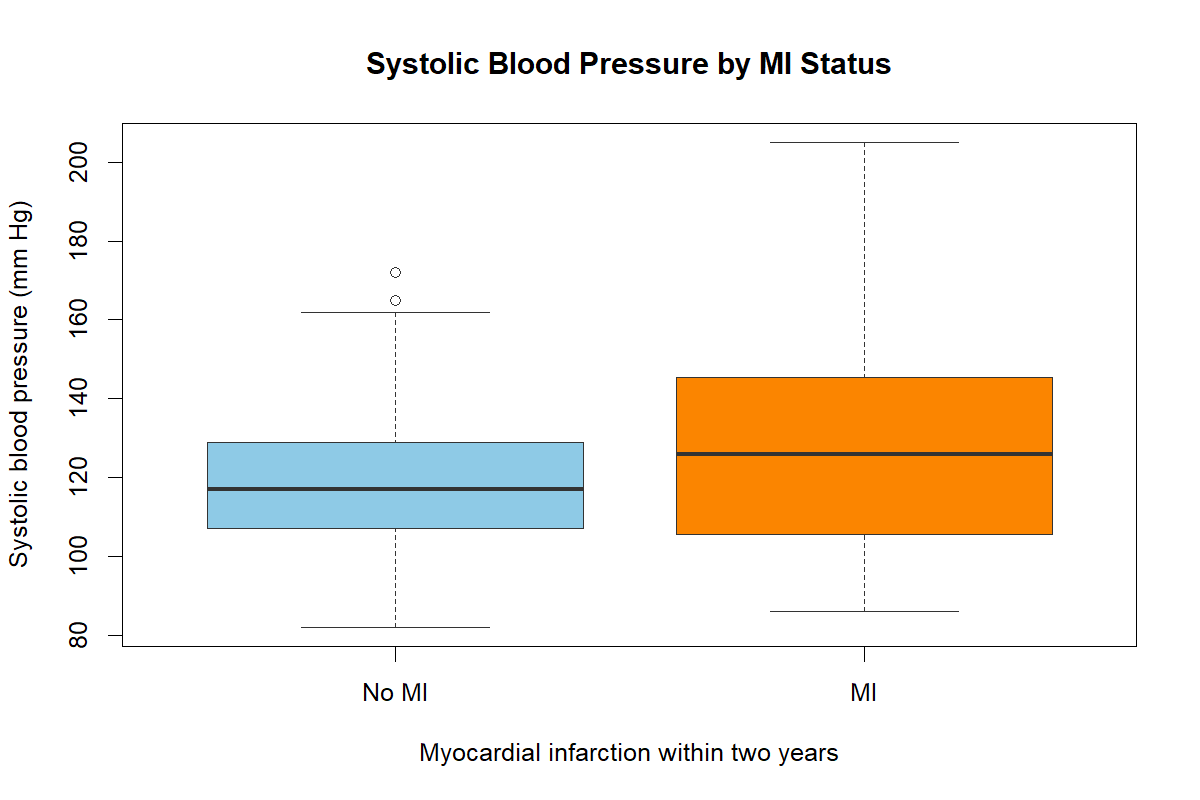
\includegraphics[
        width=\linewidth,
        height=0.53\textheight,
        keepaspectratio
      ]{code/hw2_problem1e_base_boxplot.png}

      \small\textbf{Base R:} \texttt{boxplot()}
    \column{0.49\textwidth}
      \centering
      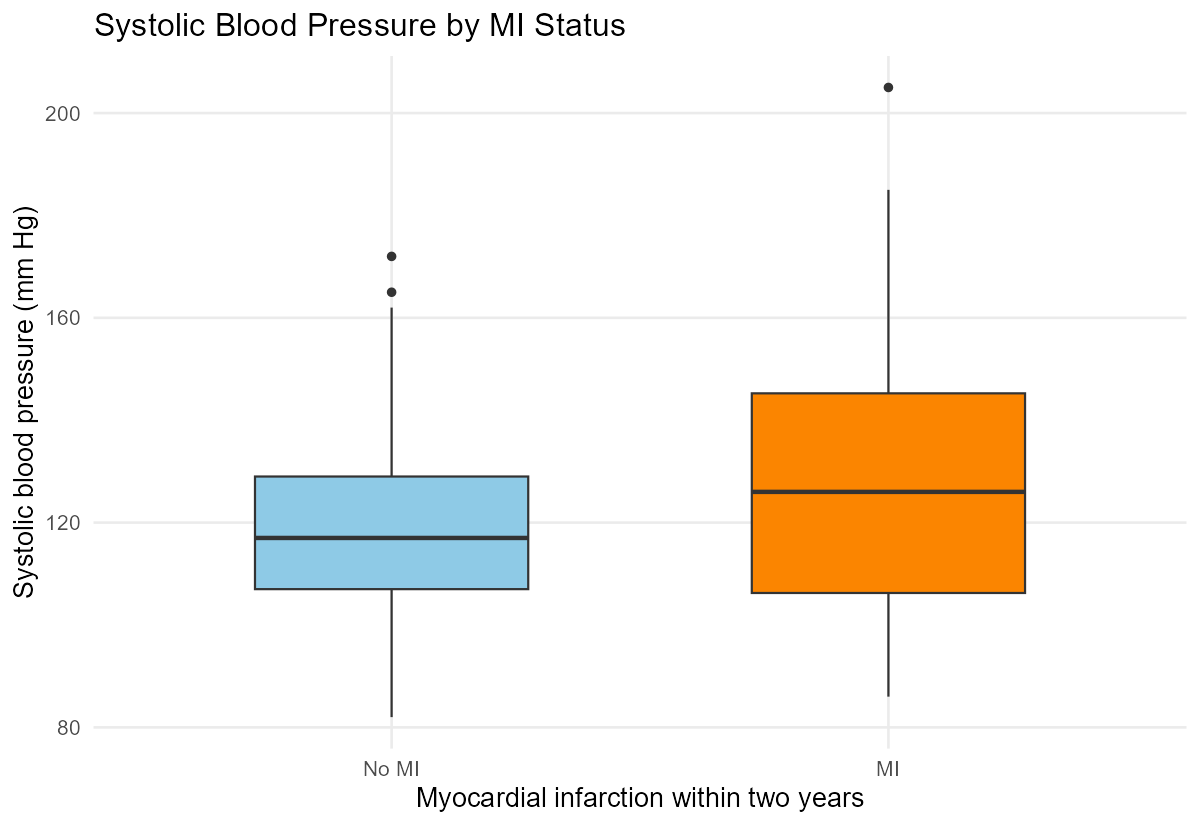
\includegraphics[
        width=\linewidth,
        height=0.53\textheight,
        keepaspectratio
      ]{code/hw2_problem1e_ggplot_boxplot.png}

      \small\textbf{ggplot2:} \texttt{geom\_boxplot()}
  \end{columns}
  \vfill
  \begin{alertblock}{Comparison}
    SBP tends to be higher in the MI group: its median is 126 mm Hg,
    compared with 117 mm Hg in the no-MI group, and its upper tail extends farther.
  \end{alertblock}
\end{frame}

\begin{frame}{Boxplot recap: fence versus whisker}
  Let \(L\) and \(U\) denote the lower and upper edges of the box.
  \[
    \operatorname{IQR}=U-L,
    \qquad
    F_L=L-1.5\operatorname{IQR},
    \qquad
    F_U=U+1.5\operatorname{IQR}.
  \]
  \begin{columns}[T,onlytextwidth]
    \column{0.48\textwidth}
      \begin{block}{What is drawn?}
        \begin{itemize}
          \item Box: from \(L\) to \(U\)
          \item Line inside the box: median
          \item Points beyond the whiskers: potential outliers
        \end{itemize}
      \end{block}
    \column{0.49\textwidth}
      \begin{block}{Whisker endpoints}
        \[
          W_L=\min\{x_i:x_i\geq F_L\},
        \]
        \[
          W_U=\max\{x_i:x_i\leq F_U\}.
        \]
      \end{block}
  \end{columns}
  \begin{alertblock}{Key distinction}
    A fence is a calculated cutoff; a whisker ends at an observed value.
    They are equal only if an observation happens to lie exactly on the fence.
  \end{alertblock}
  \vfill
  \scriptsize Source: BIOS 662 descriptive-statistics notes, p.~62.
\end{frame}

\begin{frame}{Default calculations: base R versus ggplot2}
  \scriptsize
  For ordered observations \(x_{(1)}\leq\cdots\leq x_{(n)}\):
  \begin{columns}[T,onlytextwidth]
    \column{0.49\textwidth}
      \begin{block}{Base R \texttt{boxplot()}: Tukey hinges}
        \[
          H_L=\operatorname{median}
          \left(x_{(1)},\ldots,x_{(\lceil n/2\rceil)}\right),
        \]
        \[
          H_U=\operatorname{median}
          \left(x_{(\lfloor n/2\rfloor+1)},\ldots,x_{(n)}\right).
        \]
        If \(n\) is odd, the overall median is included in both halves.
        \[
          IQR_B=H_U-H_L,
        \]
        \[
          F_L^{B}=H_L-1.5IQR_B,
          \qquad
          F_U^{B}=H_U+1.5IQR_B.
        \]
      \end{block}
    \column{0.49\textwidth}
      \begin{block}{ggplot2: type-7 quantiles}
        For \(p\in\{0.25,0.75\}\), let
        \[
          h_p=1+(n-1)p,\quad j=\lfloor h_p\rfloor,
          \quad \gamma=h_p-j,
        \]
        \[
          Q_p=(1-\gamma)x_{(j)}+\gamma x_{(j+1)}.
        \]
        Then
        \[
          IQR_G=Q_{0.75}-Q_{0.25},
        \]
        \[
          F_L^{G}=Q_{0.25}-1.5IQR_G,
          \qquad
          F_U^{G}=Q_{0.75}+1.5IQR_G.
        \]
      \end{block}
  \end{columns}
  \vspace{0.2em}
  \alert{Same \(1.5\times IQR\) convention, but different default box edges.}
\end{frame}

\begin{frame}{Why the MI-group boxplots differ}
  \small
  \begin{center}
    \begin{tabular}{lrr}
      \toprule
      \textbf{Quantity} & \textbf{Base R} & \textbf{ggplot2} \\
      \midrule
      Lower box edge & 105.50 & 106.25 \\
      Median & 126.00 & 126.00 \\
      Upper box edge & 145.50 & 145.25 \\
      IQR / box length & 40.00 & 39.00 \\
      Lower fence & 45.50 & 47.75 \\
      Upper fence & 205.50 & 203.75 \\
      Upper whisker & 205 & 185 \\
      Is 205 an outlier? & No & Yes \\
      \bottomrule
    \end{tabular}
  \end{center}
  \begin{alertblock}{Interpretation}
    In base R, \(205\leq205.50\), so the whisker reaches 205.
    In ggplot2, \(205>203.75\), so 205 is plotted separately and the whisker
    stops at the next-largest observation, 185.
  \end{alertblock}
  \vfill
  For the no-MI group, both defaults give the same box edges and whiskers.
\end{frame}

\end{document}
